\scanpage{33}
\margin{\begin{tabular}{c}
IBM\\IBM\\IBM\\IBM\\IBM\\IBM\\IBM\\IBM\\IBM\\IBM\\IBM\\IBM\\IBM\\IBM\\IBM\\IBM\\IBM\\IBM\\IBM\\IBM\\IBM\\IBM\\IBM\\IBM\\IBM\\IBM\\IBM\\IBM\\IBM\\IBM\\IBM
\end{tabular}}
\diagram{\begin{tikzcd}[ampersand replacement=\&,column sep=small,row sep=small]
1 \arrow[dr,dash] \& 1 \arrow[dr,dash]\\
1 \arrow[r] \& \pi_1(\overline X_{\unsure{\xi|g}}\setminus S_\nu) \arrow[r] \arrow[dr] \& \pi_1(\overline X_{\unsure{j|\xi}}S_\nu) \arrow[r] \arrow[dr] \& 1 \arrow[dr]\\
\&1 \arrow[r] \& \pi_1(\overline M_{g,\nu+1}) \arrow[r] \arrow[dr] \& \pi_1(M_{g,\nu+1}) \arrow[r] \arrow[dr] \& \Gamma \arrow[r,phantom,"{\unsure{\longleftarrow|\longrightarrow}}" description] \arrow[dr] \&1\\
\&\&1 \arrow[r] \& \pi_1(\overline M_{g,\nu}) \arrow[r] \arrow[dr] \& \pi_1(M_{g,\nu}) \arrow[r] \arrow[dr,Rightarrow] \& \Gamma \arrow[r,phantom,"{\unsure{\longrightarrow|\relbar}}" description] \arrow[dr,Rightarrow] \&1\\
\&\&\&\&1\&1\&1
\end{tikzcd}}
\diagram{\begin{tikzcd}[ampersand replacement=\&,column sep=small,row sep=small]
1 \arrow[dr,dash] \&1 \arrow[dr]\\
1 \arrow[r] \& \begin{gathered}\widehat{\pi}_{g,\nu}\\[-.25ex]\makebox[0pt][c]{\hspace{-3.4em}$\deleted{\unsure{1}\mathbin{-}\unsure{\pi_{g,\nu}(X)|\pi_1(X)}}$}\end{gathered} \arrow[r,"\sim"] \arrow[dr] \& \widehat{\pi}_{g,\nu} \arrow[r] \arrow[dr] \&1 \arrow[dr,dash]\\
\&1 \arrow[r] \& \widehat{\mathcal T}_{g,\nu+1} \arrow[r] \arrow[dr] \& \operatorname{Autlac}^{\circ}(\widehat{\pi}_{g,\nu})^{!} \arrow[r] \arrow[dr] \& \Gamma \arrow[r] \arrow[dr,phantom,"{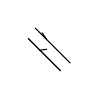
\begin{tikzpicture}[x=.65cm,y=.65cm,line cap=round,baseline=-.15cm]\draw (0,.58)--(.68,-.10);\draw (-.14,.38)--(.49,-.25);\draw (.22,.36)--(.13,.49);\draw (.09,.15)--(.22,.17);\end{tikzpicture}}" description] \&1\&\hspace{1.7em}\Sigma_{\nu+1}\\
\&\&1 \arrow[r] \& \widehat{\mathcal T}_{g,\nu} \arrow[r] \arrow[dr] \& \operatorname{Autextlac}^{\circ}(\widehat{\pi}_{g,\nu})^{!} \arrow[r,"{\text{traces}}"'] \arrow[dr] \&\Gamma \arrow[r,dash] \&1\&\hspace{1.7em}\Sigma_\nu\\
\&\&\&\&1\&1
\end{tikzcd}}
\[
\begin{gathered}
M'_{g,\nu}(K)\ni\xi\\
\mathcal T'_{g,\nu}\ni G_\xi
\end{gathered}
\]
\diagram{\ensuremath{\begin{array}{@{}r@{\;}c@{\qquad\qquad}c@{}}
\deleted{\unsure{\Gamma_g|\Sigma_g}}&&\\
&\widehat\Sigma_{g,\nu}^{\sim}&\Sigma_{g,\nu}\\
&\Vert&\\
&\overline\Sigma_{g,\nu}&
\end{array}}}
\margin{\begin{tabular}{c}6\\5\\4\\3\\2\\1\\0\end{tabular}}
\margin{2975 -- 132}
\mspage{32}
